\section{Patterns in Bit Error Distributions}
\label{sec:bit_error_patterns}

We designed two experiments to investigate the results of Schmidt~\etal~\cite{Schmidt2013}.
The first experiment was used to confirm their findings and also investigate the influence of hardware layout on \ac{BER} patterns, while the second experiment investigated the influence of temperature on these patterns.

\subsection{Effects of Board Layout}
\label{subsec:effects_of_board_layout}

In all our experiments we used Tmote Sky motes, which are commercial drop-in replacements for the original Telos mote design by Polastre~\etal~\cite{Polastre2005}.
We had hardware revisions available from two manufacturers: the original design from (now defunct) MoteIV Corporation and the Maxfor MTM-CM5000MSP, which uses a slightly different schematic and board layout.
Notable differences include the \SI{3}{\volt} regulator and the physical layout of the radio circuitry.

In the experiment a pair of CM5000 and original motes transmitted to two CM5000 and two original motes.
All motes were powered by the on-board voltage regulator via the USB connector, which was also used to establish serial communications with the PC.
This redundant placement shown in Figure~\ref{fig:8mote_experiment_setup} was chosen so that the same transmission was received by both types.
Over the course of six days the four transmitters sent 563,500 messages each, totaling 2,254,000 transmitted messages at power setting 2 (below \SI{-25}{\dBm}).
Since each transmission was sent to four receivers, a total of 9,016,000 receptions should have been possible.
Of those 5,280,369 were received and 2,497,744 had at least one bit error.
The experiment was located in the large climate-controlled server room in the basement, where the temperature remained within $20$--\SI{25}{\celsius} with no other changes in the environment.

\begin{figure}[t]
	\centering
	\begin{tikzpicture}
		\newcommand\receiver[5]{%
		    \begin{scope}[xshift=#1cm,yshift=#2cm,rotate=#3]
		        \draw[fill=#4] (0,0) rectangle (1,2.1);
		     	\draw[fill=black!10] (0.33,0.1) rectangle (0.66,-0.45);
		     	\draw[snake=snake, white, segment amplitude=1.75, segment length=5, line width=1.25pt] (0.1, 1.95) -- (0.9, 1.95);
		     	\node at (0.5cm, 1.05cm) {#5};
		    \end{scope}
		}
		\newcommand\transmitter[5]{%
			\receiver{#1}{#2}{#3}{#4}{#5};
		    \begin{scope}[xshift=#1cm,yshift=#2cm,rotate=#3]
		     	\draw[snake=expanding waves, segment angle=40, segment length=7] (0.5,2) -- (0.5,3);
		    \end{scope}
		}

		% new = red, old = blue
		% new transmitter
		\transmitter{3}{7}{-65}{motered}{0};
		\transmitter{3.675}{5.5}{-65}{motered}{1};		

		% new transmitter
		\transmitter{0}{2}{-65}{moteblue}{2};
		\transmitter{0.675}{0.5}{-65}{moteblue}{3};

		\receiver{13}{0}{180}{motered}{7};
		\receiver{13}{3}{180}{moteblue}{6};
		\receiver{13}{6}{180}{motered}{5};
		\receiver{13}{9}{180}{moteblue}{4};

		% labels
		\node at (3, 7.75) {CM5000};
		\node at (0, 2.8) {Original};

		\node at (3, -1.5) {Transmitters};
		\node at (10.5, -1.5) {Receivers};
	\end{tikzpicture}
	\caption{Experiment setup with four transmitters and four receivers.}
	\label{fig:8mote_experiment_setup}
\end{figure}

The CM5000 motes required to be physically closer to the receivers at the same power setting to have similar link quality as the original motes.
This might be hinting at a difference in range between the two hardware layouts, however, our experiment was not set up to systematically investigate range.

In the initial evaluation we noted some significant differences in the quality of some links, where the co-located transmitters are sending to the same receiver.
For example, the link 3--5 is of very good quality with over 99\% \ac{PRR}, however link 2--5 shows quite the opposite with less than 1\% \ac{PRR}, even though both transmitters are located at the same distance and angle from the receiver.
This confirms the findings of Baccour~\etal~\cite{Baccour2012}, specifically that link quality is anisotropic, \ie the communication range exhibits a non-spherical pattern.
More exhibitions of this behavior can be found in the complete table of link qualifiers in the Appendix as Table~\ref{tab:8mote_link_qualities}.

Further analysis revealed the same bit and symbol error patterns as first discovered by Schmidt~\etal~\cite{Schmidt2013}, which state that within any transmitted symbol, the first three \acp{MSB} are more likely to break than the \ac{LSB} and that symbols 8--15 with the \ac{MSB} set to 1 are more likely to break than 0--7.
The normalized occurance of bit errors are plotted in Figure~\ref{fig:8mote_bit_errors}, with the first 12 bytes (96 bits) consisting of the message header with partially fixed content and the remaining 80 bytes are the constant payload, made up of two 32 byte patterns of 0x0000, 0x1111, $\ldots$ 0xFFFF, and one 16 byte pattern of 0x00, 0x11, $\ldots$ 0xFF.

\begin{figure}[t]
	\subfigure[XL] {
    	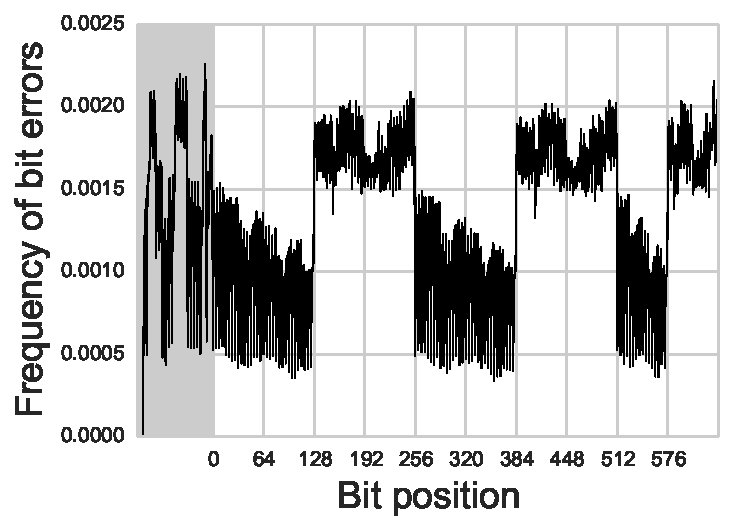
\includegraphics[width=0.475\columnwidth]{figures/8mote_0-5_xor}
    	\label{fig:8mote_bit_errors_xl}
    }
    \subfigure[L] {
	    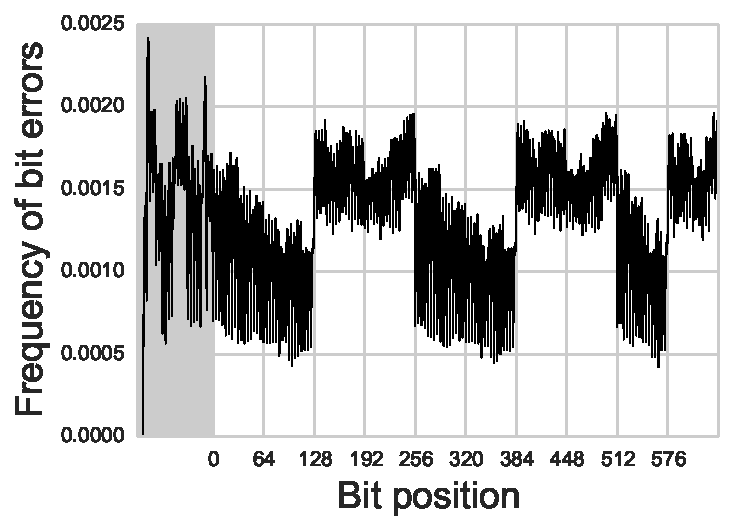
\includegraphics[width=0.475\columnwidth]{figures/8mote_1-6_xor}
	    \label{fig:8mote_bit_errors_l}
	}
	\subfigure[M] {
	    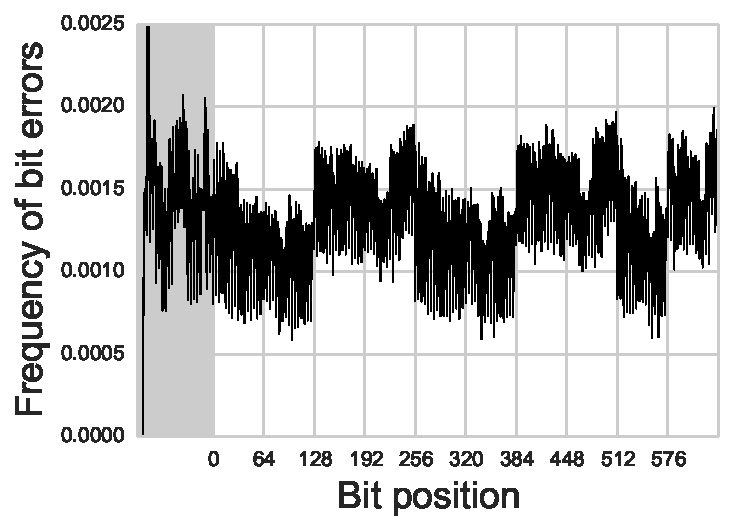
\includegraphics[width=0.475\columnwidth]{figures/8mote_2-6_xor}
	    \label{fig:8mote_bit_errors_m}
	}
	\subfigure[S] {
	    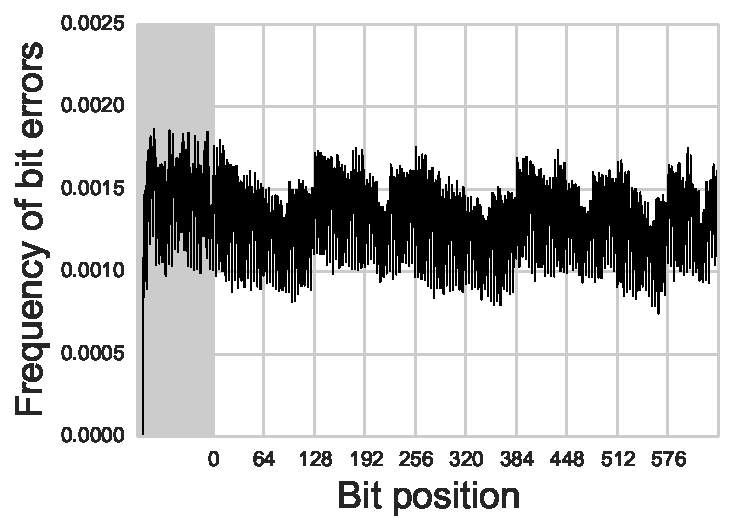
\includegraphics[width=0.475\columnwidth]{figures/8mote_2-7_xor}
	    \label{fig:8mote_bit_errors_s}
	}
	\caption{Four magnitudes of \acs{BER} patterns with fixed payload of twice 0x0000, 0x1111, $\ldots$ 0xFFFF and once 0x00, 0x11, $\ldots$ 0xFF. The message header is indicated in gray.}
	\label{fig:8mote_bit_errors}
\end{figure}

We were able to confirm the findings of Schmidt~\etal{} and extend them with a classification of the influence of symbols on \ac{BER}.
The Subfigures in \ref{fig:8mote_bit_errors} show four magnitudes of this phenomenon, ranging from an extreme to almost no difference between symbols, named XL, L, M and S.
The remaining links can be classified into these four categories as done in Table~\ref{tab:8mote_bit_error_link_classification}.
XL and L patterns seems to be more common than M and S, with 8 vs. 3 links respectively, however, the table is incomplete, since only 11 out of 16 links had enough bit errors to recognize and categorize the pattern.

Schmidt~\etal{} also looked into the burstiness of errors and showed in their research that burst errors are not independently distributed.
The authors explained the drop from 4-bit bursts to 5-bit bursts with the added difficulty of corrupting a minimum of 7 bits to overcome the minimum Hamming distance of 12 between two symbol's chip sequences.
They also hypothesized that a similar drop would occur between 8-bit and 9-bit bursts, but were unable to confirm this, due to their limited sample size.
With our larger sample size we can confirm their hypothesis, with the drop quite noticeable in Figure~\ref{fig:8mote_xl_burst}.

\begin{table}[ht]
	\begin{tabularx}{\linewidth}{|c*{4}{|c}|}
	\hline
	\T \cellcolor{slightgray} Receiver	& \multicolumn{1}{X|}{\cellcolor{motered} \centering Sender 0} & \multicolumn{1}{X|}{\cellcolor{motered} \centering Sender 1} & \multicolumn{1}{X|}{\cellcolor{moteblue} \centering Sender 2}	& \multicolumn{1}{X|}{\cellcolor{moteblue} \centering Sender 3}\\
	\hline

	\cellcolor{moteblue}\T 4 & S  & \cellcolor{slightgray} & \cellcolor{slightgray} & \cellcolor{slightgray}   \B\\
	\hline
	\cellcolor{motered}\T  5 & XL & XL & L & XL \B\\
	\hline
	\cellcolor{moteblue}\T 6 & XL & L  & M & \cellcolor{slightgray}   \B\\
	\hline
	\cellcolor{motered}\T  7 & L  & \cellcolor{slightgray} & S & L  \B\\
	\hline 
	\end{tabularx}

	\caption{Classification of all links with enough absolute bit errors (otherwise gray).}
	\label{tab:8mote_bit_error_link_classification}
\end{table}

\begin{figure}[t]
	\subfigure[XL burst error distribution.] {
    	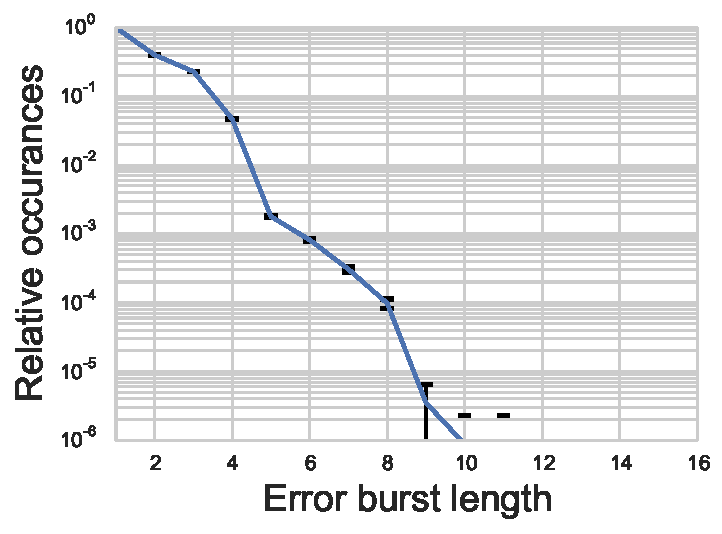
\includegraphics[width=0.475\columnwidth]{figures/8mote_0-5_burst}
    	\label{fig:8mote_xl_burst}
    }
    \subfigure[S burst error distribution.] {
	    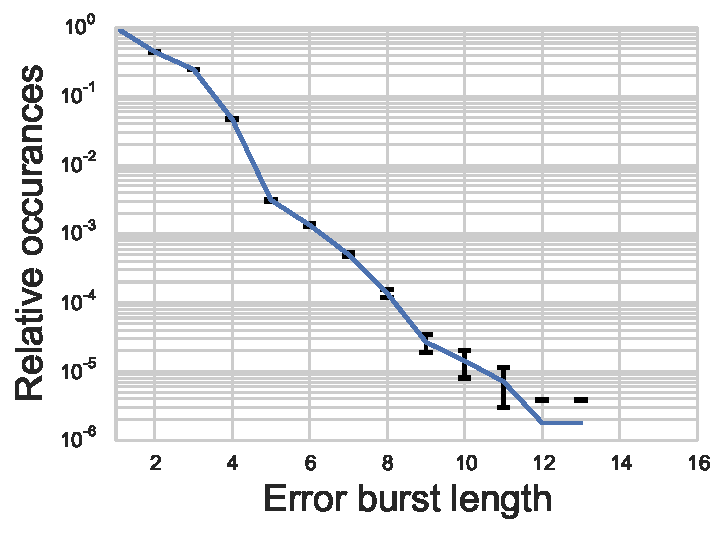
\includegraphics[width=0.475\columnwidth]{figures/8mote_2-7_burst}
	    \label{fig:8mote_s_burst}
	}
	\caption{The burst error distributions of XL and S magnitudes show more longer burst errors in S magnitude. The error bars denote 99\% confidence intervals.}
	\label{fig:8mote_burst_error}
\end{figure}

We cannot see any correlation between the four \ac{BER} pattern classifications and burst error distribution or any other variable.
We therefore believe the magnitude of these patterns to be a result of the analog circuits of the radio, something that cannot be changed or improved by software.

\subsection{Effects of Temperature}
\label{subsec:effects_of_temperature}

To investigate the influence of temperature on \ac{BER} patterns, we used the CM5000 motes in the temperature boxes as described in Section~\ref{sec:temperature_box}.
To minimize signal disturbance we mounted the boxes in the storage room on wooden posts, so that they were floating in free space.
We placed the boxes at a fixed distance of \SI{280}{\centi\metre} to each other and controlled link quality sorely by rotating the antenna.

We ran three experiments with the same constant payload as described in the Subsection~\ref{subsec:effects_of_board_layout} but with power setting 3 (\SI{-25}{\dBm}) at \SI{30}{\celsius}, \SI{50}{\celsius} and \SI{70}{\celsius}.
Due to the decrease of link quality at higher temperatures, discussed in detail in Section~\ref{sec:packet_reception_rate}, we had to adjust mote rotation to regulate \ac{BER} at these temperatures, therefore small differences in absolute bit errors are present.
However, Figure~\ref{fig:temperature_bit_errors} shows no significant difference between \ac{BER} patterns at all three temperatures and therefore we did not pursuit this further.

\begin{figure}[t]
	\subfigure[\acs{BER} pattern at \SI{50}{\celsius}.] {
    	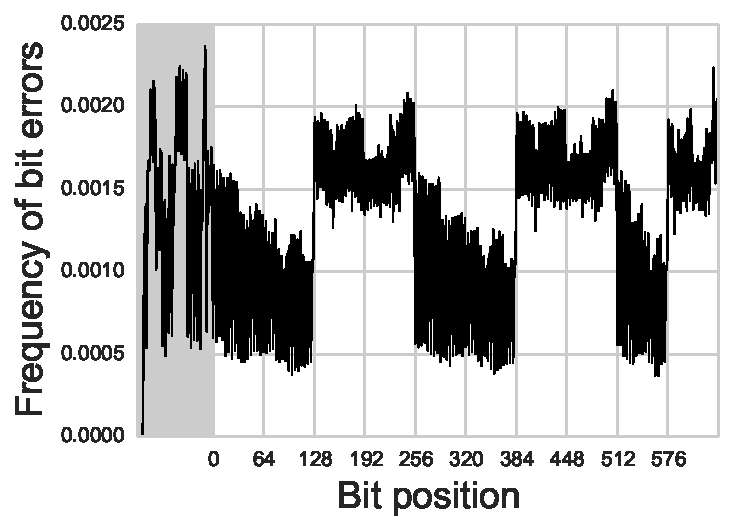
\includegraphics[width=0.475\columnwidth]{figures/temperature_1_5}
    	\label{fig:temperature_bit_errors_30}
    }
    \subfigure[\acs{BER} pattern at \SI{70}{\celsius}.] {
	    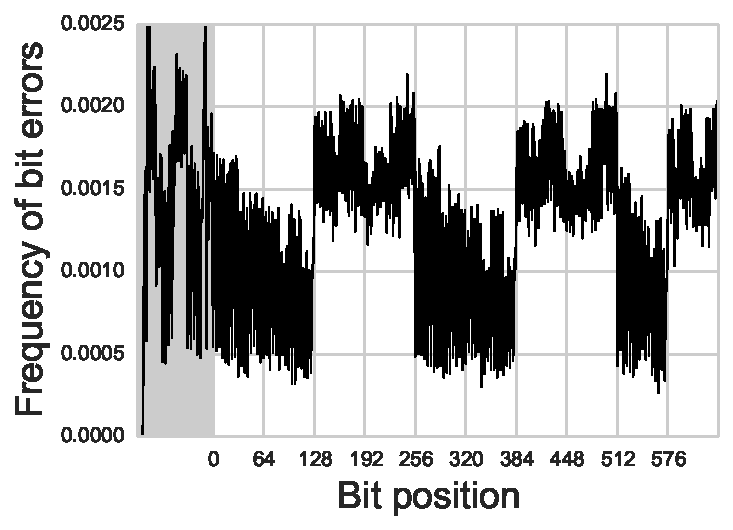
\includegraphics[width=0.475\columnwidth]{figures/temperature_0_6}
	    \label{fig:temperature_bit_errors_70}
	}
	\caption{\acl{BER} patterns show no difference between \SI{30}{\celsius}, \SI{50}{\celsius} and \SI{70}{\celsius}. The pattern at \SI{30}{\celsius} is omitted, since it is redundant.}
	\label{fig:temperature_bit_errors}
\end{figure}


\subsection{Pattern Anomalies}
\label{subsec:pattern_anomalies}

Even though the vast majority of experiment evaluations confirmed these patterns, there were two runs with  drastically different outcome.
We were very surprised to find a second, completely opposite \ac{BER} pattern as shown in Figure~\ref{fig:anomalie_bit_error}.
Here the symbols 0-7 show a higher average \ac{BER} and a less pronounced 4-bit saw-tooth pattern than symbols 8-15.
The pattern almost looks like an ``inverse'' of those described earlier.

The first time it occurred, we attributed this to influences of the environment and discarded it.
Two months later, this pattern occurred again with different hardware in a different setup in a different environment.
Both times, the motes were exposed to high temperature (>\SI{70}{\celsius}) over several hours, however, we were unable to confirm if this indeed triggered the pattern.
This pattern remained for days, regardless of temperature, link quality or message payload.

We cannot envision a source of interference capable of fundamentally changing this \ac{BER} distribution and neither does a permanent change of the radio chip's hardware at high temperature seem possible.
The CC2420 radio is rated to be operated at temperatures up to \SI{85}{\celsius} and to be stored at up to \SI{150}{\celsius}, while our experiments where limited to at most \SI{90}{\celsius} for a few hours.

Since we could not find any other reference to this pattern in literature and due to the rarity of this occurrence in our experiments and the difficulty of its repeatability, we decided to focus on investigating the ``normal'' patterns.

\begin{figure}[t]
	\subfigure[First occurance.] {
    	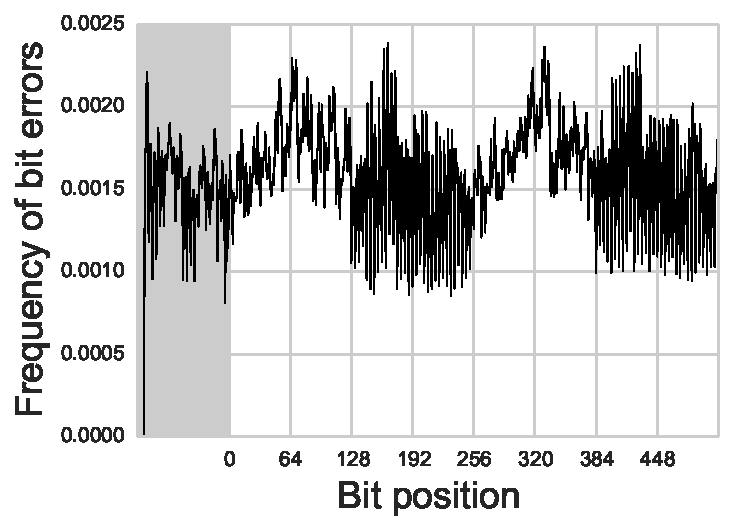
\includegraphics[width=0.475\columnwidth]{figures/anomaly_first}
    	\label{fig:anomalie_earlier}
    }
    \subfigure[Second occurance.] {
	    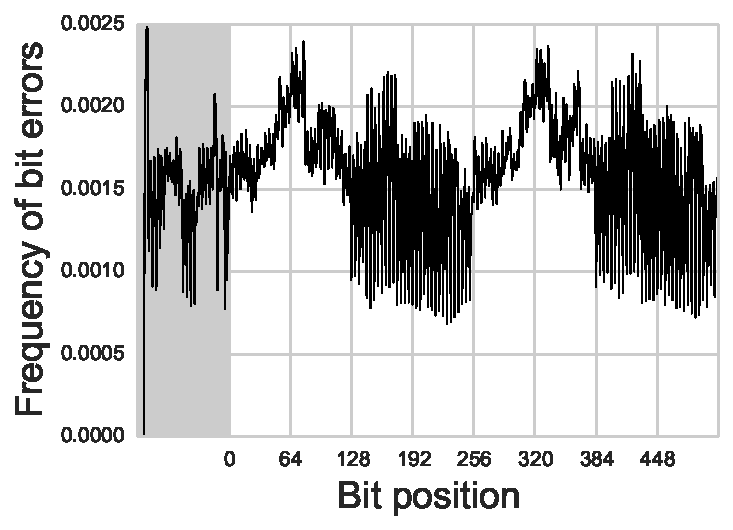
\includegraphics[width=0.475\columnwidth]{figures/anomaly_second}
	    \label{fig:anomalie_later}
	}
	\caption{``Inverted'' \acs{BER} pattern anomaly of constant data. Only the first two 32 byte patterns are shown.}
	\label{fig:anomalie_bit_error}
\end{figure}


